\chapter{Opis projektnog zadatka}
		
		\textbf{\textit{dio 1. revizije}}\\
		
		\textit{Na osnovi projektnog zadatka detaljno opisati korisničke zahtjeve. Što jasnije opisati cilj projektnog zadatka, razraditi problematiku zadatka, dodati nove aspekte problema i potencijalnih rješenja. Očekuje se minimalno 3, a poželjno 4-5 stranica opisa.	Teme koje treba dodatno razraditi u ovom poglavlju su:}
		\begin{packed_item}
			\item \textit{potencijalna korist ovog projekta}
			\item \textit{postojeća slična rješenja (istražiti i ukratko opisati razlike u odnosu na zadani zadatak). Dodajte slike koja predočavaju slična rješenja.}
			\item \textit{skup korisnika koji bi mogao biti zainteresiran za ostvareno rješenje.}
			\item \textit{mogućnost prilagodbe rješenja }
			\item \textit{opseg projektnog zadatka}
			\item \textit{moguće nadogradnje projektnog zadatka}
		\end{packed_item}
		
		\textit{Za pomoć pogledati reference navedene u poglavlju „Popis literature“, a po potrebi konzultirati sadržaj na internetu koji nudi dobre smjernice u tom pogledu.}\\

		\textbf{Donori Krvi}\\

		Naš zadatak svodi se na izradu programske potpore za web aplikaciju (trenutno nema ime) koja će služiti tome da svim donorima i zaposlenicima Hrvatskog Crvenog Križa olakša neke akcije vezane uz darivanje krvi.

		Ukratko, koristeći našu aplikaciju, korisnici zainteresirani za davanje krvi moći će se prijaviti u sustav, pregledavati sve aktivne lokacije davanja krvi, prijavljivati se na njih, rezervirati termine i pregledavati neke osnovne informacije o aplikaciji i Hrvatskom Crvenom Križu te o podacima svog profila.

		Zaposlenici Hrvatskog Crvenog Križa moći će pregledavati koliko ljudi će prisustvovati određenoj akciji i moći će upisivati sva darivanja koja će se prikazivati na našoj aplikacji. Moći će organizirati i uređivati povremene akcije darivanja krvi koje se mogu održati na bilo kojoj lokaciji, i najvažnije, hitnom porukom moći će obavijestiti sve korisnike o nedostatku krvi na određenom području.

		Cilj ove aplikacije je modernizirati spremanje i prikaz podataka vezanih uz darivanje krvi, automatizirati i olakšati proces naručivanja, pa tako i skratiti vrijeme čekanja u redu, automatizirati proces izdaje potvrda nakon određenog broja darivanja i pružiti korisnicima informacije vezane uz moguća mjesta darivanja krvi pa tako i povećati volumen darovane krvi. 

		Lokacije na kojima je moguće dati krv sastoje se od dva tipa lokacija zasnovanih na stalnosti termina darivanja krvi:
		\begin{packed_enum}

					\item Zdravstvene ustanove sa stalnim terminima
					\item Lokacije privremenih akcija koje organizira Hrvatski Crveni Križ

		\end{packed_enum}

		U prvu kategoriju spadaju KBC Osijek, KBC Rijeka, KBC
		Split, OB Dubrovnik, OB Varaždin, OB Zadar i Hrvatski zavod za transfuzijsku medicinu Zagreb. 

		Korisnici koji će koristiti našu aplikaciju dijele se u dvije kategorije: nerigistrirani korisnik (gost) i registrirani korisnik. Nadalje, korisnik može registrirati dvije vrste računa: Donor krvi i Zaposlenik Hrvatskog Crvenog Križa (administrator, admin). Potreba za ove modele korištenja aplikacije proizlazi iz toga što dio aplikacije treba biti vidljiv i još neprijavljenim korisnicima te toga što prosječan donor krvi i zaposlenik Hrvatskog Crvenog Križa koriste aplikaciju na znatno različite načine.

		\begin{packed_item}
				\item \textbf{Gost} - način korištenja aplikacije kada korisnik nije prijavljen u sustav. U ovom način moguće je prijaviti se ili registrirati novi korisnički račun. Osim toga, moguć je pregled svih lokacija vađenja krvi, i onih stalnih i trenutno aktivnih povremenih akcija, ali bez mogućnosti naručivanja termina. Također, gostu je dostupna stranica s osnovnim informacijama o aplikaciji i Hrvatskom Crvenom Križu.
				\item \textbf{Donor krvi} - kad se gost prijavi u sustav, jedna od mogućih opcija je napraviti račun kao donor krvi. U ovom načinu korištenja aplikacije korisnik može napraviti sve što i gost, s još dodatnim funkcionalnostima. Kod pregleda lokacija, prikazuje mu se gumb koji ga vodi na odabir i rezervaciju termina. Dostupna mu je i mogućnost pregleda vlastitog profila s brojnim informacijama koje ćemo detaljno navesti kasnije. Također, kad admin pošalje obavijest za hitnom akcijom, korisnik dobiva poruku na mail. Kad klikne na link u mailu ili pristupi aplikaciji nakon poziva, preusmjerit će se na stranicu na kojoj ima mogućnost rezervirati termin za hitnu akciju.
				\item \textbf{Administrator} - dalje u tekstu nazvan i Hrvatski Crveni Križ ili samo Crveni Križ. Također ima sve opcije iste kao i gost s još nekim dodatnim mogućnostima. Admin verificira korisnika koji se registrira, nakon čega se korisnik može prijaviti u sustav. Također, dodaje, mijenja i arhivira akcije darivanja krvi. Može napraviti zapis svaki put kad netko daruje krv u svrhu praćenja povijesti darivanja krvi svakog korisnika. Može vidjeti koliko ljudi je rezerviralo termin za neku akciju.
		\end{packed_item}

		Naša web aplikacija zamišljena je kao skupina raznih stranica koje će nam pomoći kod organizacije svih funkcionalnosti koje aplikacija treba imati. Registracija korisnika od gosta traži sljedeće informacije:

		\begin{packed_item}
				\item Ime i prezime
				\item Spol
				\item Adresa
				\item Primarna zdravstvena ustanova
				\item Email adresa
				\item Datum rođenja
				\item MBO
				\item Krvna grupa
		\end{packed_item}

		Jednom kad se osoba odluči registrirati, svi upisani podaci šalju se adminu na verifikaciju. Nakon što admin pregleda podatke i zaključi da izgledaju ispravno, potvrđuje podatke i njegov račun postaje aktivan. Korisnik dobiva mail da ima mogućnost prijaviti se u aplikaciju. 

		Kad se korisnik prijavi, prvo što vidi na stranici je prikaz svojeg profila. Na njemu su vidljive sve njegove osobne informacije, od kojih neke može i uređivati. Vidljive su mu sve aktivne rezervacije koje onda može otkazati ako je potrebno. Sljedeće što je vidljivo prijavljenom korisniku jest povijest svih termina kad je darovao krv i admin je to upisao u aplikaciju. I na kraju, vidljiva mu je lista svih potvrda koje može "osvojiti" ako dovoljan broj puta da krv. 

		Kretanjem kroz meni koji se nalazi na svakoj stranici aplikacije, korisnik se može prebaciti na stranicu za pregledavanje lokacija na kojima ima mogućnost prijaviti termin za davanje krvi. Sve lokacije na stranici također su vidljive na karti. Odabirom lokacije korisnik je preusmjeren na biranje termina i klikom na gumb potvrđuje rezervaciju. 

		Tijekom registracije gost ima mogućnost registrirati se kao zaposlenik Hrvatskog Crvenog Križa. Nakon što je verificiran, prijavom u sustav ovaj korsinik postaje admin. Može verificirati ostale goste koji se žele registrirati. Može stvoriti novu akciju unoseći lokaciju, termine i trajanje akcije. Ako je nešto slučajno krivo unio, ima mogućnost urediti akciju. 

		Akcije koje admin stvara imaju dva stanja:

		\begin{packed_item}
				\item aktivne - akcija je stvorena i još nije istekla. Vidljiva je svim korisnicima i admin ju može uređivati ako je potrebno.
				\item arhivirane - akcija je "istekla" i više nije vidljiva korisnicima. Admin ju više ne može uređivati, ali ju može pregledavati.
		\end{packed_item}

		Sve akcije počinju kao aktivne. Kad prođe zadnji dan akcije, ona se automatski arhivira. Ako iz nekog razloga admin treba zatvoriti akciju prije dana isteka, ponuđena mu je mogućnost to napraviti.


		Admin također u slučaju nestanka zaliha neke krvne grupe može poslati korisnicima obavijest za hitnu akciju darivanja krvi. Upisom krvne grupe i lokacije u odgovarajuće prozore prvo šalje svim korisnicima u krugu od 20km poruku na mail i modal obavijest u aplikaciji. Korisnici imaju mogućnost potvrditi svoj dolazak i rezervirati termin za navedenu hitnu akciju. Ako se u određenom vremenskom roku ne prijavi dovoljno ljudi, aplikacija će poslati poruku svim ostalim korisnicima u regiji.

		Moguće nadogradnje koje bi daljnje poboljšale ovaj sustav su pregled statistike za zaposlenike Hrvatskog Crvenog Križa. To uključuje izradu posebne stranice gdje bi administratorima bilo prikazano koliko ljudi se prijavilo za koju akciju i u kojim terminima, koji su omjeri krvnih grupa prijavljenih ljudi, koliko ljudi se odazvalo na neku hitnu akciju, koliko krvi je sveukupno sakupljeno kroz različite vremenske periode i slično.



		\eject
		
		\section{Primjeri u \LaTeX u}
		
		\textit{Ovo potpoglavlje izbrisati.}\\

		U nastavku se nalaze različiti primjeri kako koristiti osnovne funkcionalnosti \LaTeX a koje su potrebne za izradu dokumentacije. Za dodatnu pomoć obratiti se asistentu na projektu ili potražiti upute na sljedećim web sjedištima:
		\begin{itemize}
			\item Upute za izradu diplomskog rada u \LaTeX u - \url{https://www.fer.unizg.hr/_download/repository/LaTeX-upute.pdf}
			\item \LaTeX\ projekt - \url{https://www.latex-project.org/help/}
			\item StackExchange za Tex - \url{https://tex.stackexchange.com/}\\
		
		\end{itemize} 	


		
		\noindent \underbar{podcrtani tekst}, \textbf{podebljani tekst}, 	\textit{nagnuti tekst}\\
		\noindent \normalsize primjer \large primjer \Large primjer \LARGE {primjer} \huge {primjer} \Huge primjer \normalsize
				
		\begin{packed_item}
			
			\item  primjer
			\item  primjer
			\item  primjer
			\item[] \begin{packed_enum}
				\item primjer
				\item[] \begin{packed_enum}
					\item[1.a] primjer
					\item[b] primjer
				\end{packed_enum}
				\item primjer
			\end{packed_enum}
			
		\end{packed_item}
		
		\noindent primjer url-a: \url{https://www.fer.unizg.hr/predmet/proinz/projekt}
		
		\noindent posebni znakovi: \# \$ \% \& \{ \} \_ 
		$|$ $<$ $>$ 
		\^{} 
		\~{} 
		$\backslash$ 
		
		
		\begin{longtblr}[
			label=none,
			entry=none
			]{
				width = \textwidth,
				colspec={|X[8,l]|X[8, l]|X[16, l]|}, 
				rowhead = 1,
			} %definicija širine tablice, širine stupaca, poravnanje i broja redaka naslova tablice
			\hline \SetCell[c=3]{c}{\textbf{naslov unutar tablice}}	 \\ \hline[3pt]
			\SetCell{LightGreen}IDKorisnik & INT	&  	Lorem ipsum dolor sit amet, consectetur adipiscing elit, sed do eiusmod  	\\ \hline
			korisnickoIme	& VARCHAR &   	\\ \hline 
			email & VARCHAR &   \\ \hline 
			ime & VARCHAR	&  		\\ \hline 
			\SetCell{LightBlue} primjer	& VARCHAR &   	\\ \hline 
		\end{longtblr}
		

		\begin{longtblr}[
				caption = {Naslov s referencom izvan tablice},
				entry = {Short Caption},
			]{
				width = \textwidth, 
				colspec = {|X[8,l]|X[8,l]|X[16,l]|}, 
				rowhead = 1,
			}
			\hline
			\SetCell{LightGreen}IDKorisnik & INT	&  	Lorem ipsum dolor sit amet, consectetur adipiscing elit, sed do eiusmod  	\\ \hline
			korisnickoIme	& VARCHAR &   	\\ \hline 
			email & VARCHAR &   \\ \hline 
			ime & VARCHAR	&  		\\ \hline 
			\SetCell{LightBlue} primjer	& VARCHAR &   	\\ \hline 
		\end{longtblr}
	


		
		
		%unos slike
		\begin{figure}[H]
			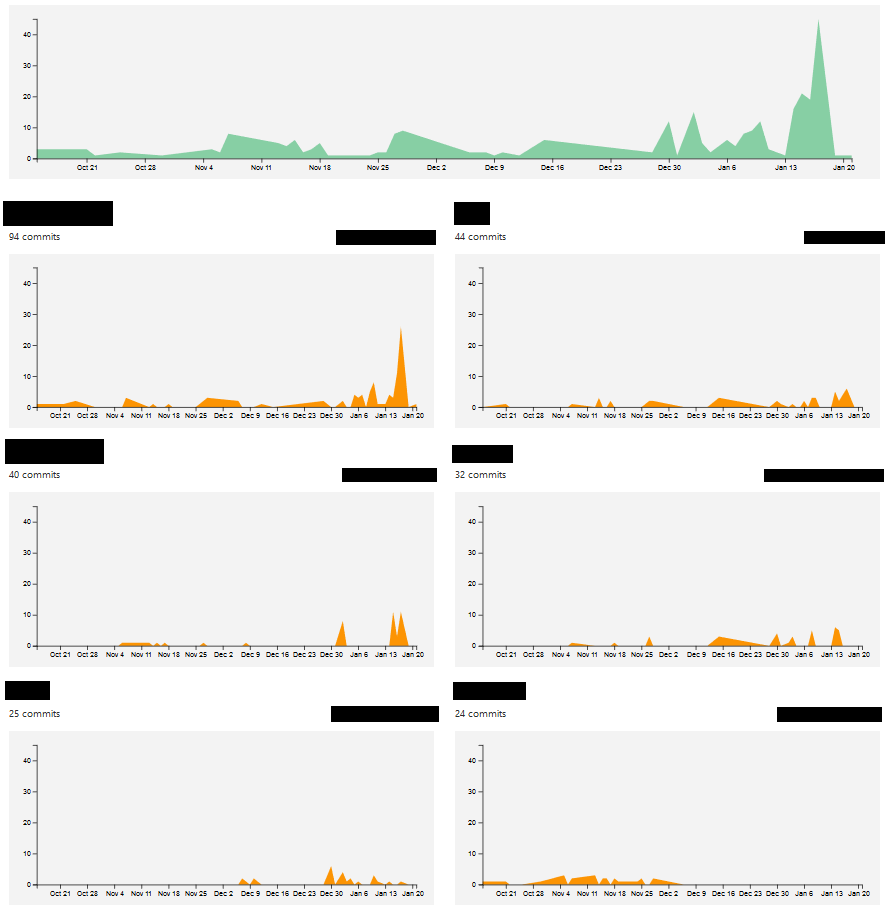
\includegraphics[scale=0.4]{slike/aktivnost.PNG} %veličina slike u odnosu na originalnu datoteku i pozicija slike
			\centering
			\caption{Primjer slike s potpisom}
			\label{fig:promjene}
		\end{figure}
		
		\begin{figure}[H]
			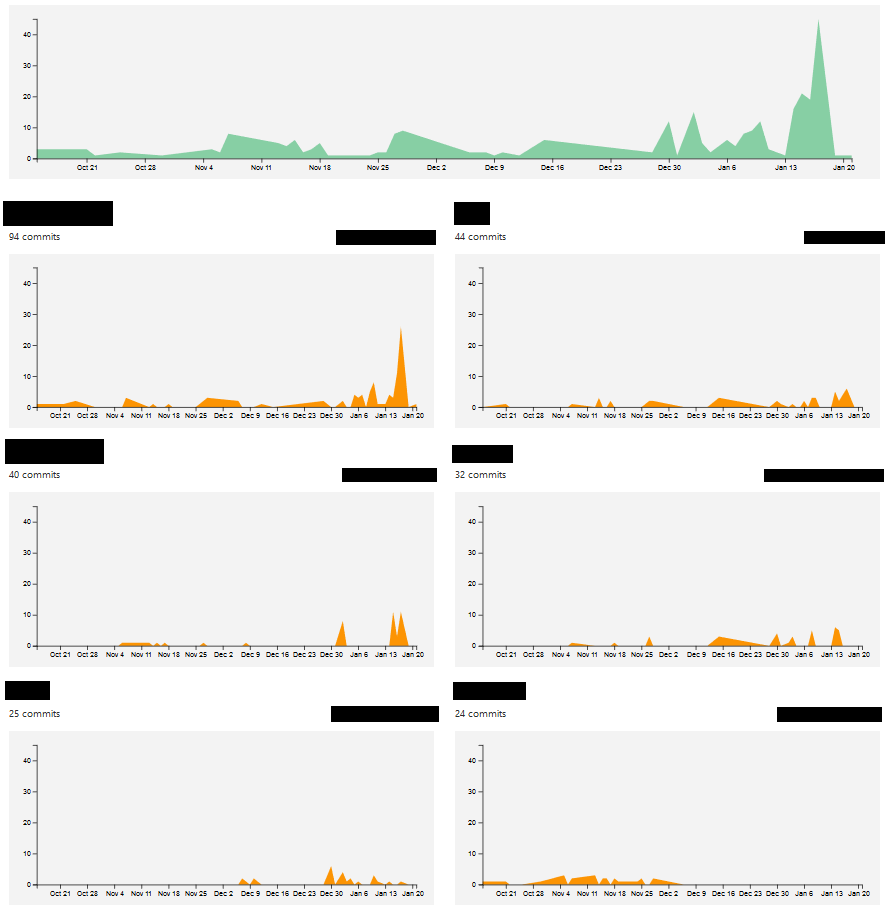
\includegraphics[width=\textwidth]{slike/aktivnost.PNG} %veličina u odnosu na širinu linije
			\caption{Primjer slike s potpisom 2}
			\label{fig:promjene2} %label mora biti drugaciji za svaku sliku
		\end{figure}
		
		Referenciranje slike \ref{fig:promjene2} u tekstu.
		
		\eject
		
	
